
% ════════════════════════════════════════════
% 曝光量回归模型（5.3）
% ════════════════════════════════════════════
\subsection{曝光量回归模型}

\subsubsection{模型设定与估计}

本部分以 log1p 曝光量为因变量，构建包含粉丝规模、帖子类型、内容主题、月份、星期、时段与付费标记的全模型，并用 HC3 协方差矩阵处理异方差。模型写作
\begin{equation}
    y_i=\boldsymbol{x}_i^{\mathrm{T}}\boldsymbol{\beta}+\varepsilon_i,
    \qquad i=1,2,\ldots,n,
\end{equation}
其中 $y_i=\log(1+Y_i)$，$\boldsymbol{\beta}$ 为待估系数，$\varepsilon_i$ 为随机扰动。系数由最小二乘估计；在经典假定下，系数协方差等于扰动方差乘以设计矩阵交叉乘积的逆。曝光量重尾使残差方差随拟合值变化，经典标准误会低估不确定性，因此采用 White 异方差稳健估计的 HC3 修正：第 $i$ 个残差平方除以 $(1-h_{ii})^2$ 后加权，$h_{ii}$ 为该观测的杠杆值\cite{white1980}。该修正不改变系数点估计，只修正标准误，系数表可以与经典结果直接对照。

为分离共线的影响，设置五个递进模型。M0 只含常数项，作为均值基线；M1 为全模型，同时含粉丝规模对数与 11 个月份哑变量；M2 剔除粉丝规模、保留月份固定效应；M3 保留粉丝规模、剔除月份；M4 同时含粉丝规模与线性月份项。M2 用月份固定效应吸收粉丝规模的累积趋势，是本报告的最终解释模型；M1、M3、M4 用于检验付费与内容类型的系数是否随设定改变。

图\ref{fig:q3_score}以评分表形式比较五种模型。评分由十折交叉验证的 $R^2$ 均值减去 0.1 倍折间标准差得到，兼顾预测精度与稳定性。M2 的得分为 0.0909，居五者之首；M4 为 0.0888、M1 为 0.0871、M3 为 0.0848，均值基线 M0 为 $-0.0238$。M2 的样本内 $R^2$ 为 0.2068、调整 $R^2$ 为 0.1650、残差标准误 1.0765，十折交叉验证 $R^2$ 为 0.1010、RMSE 1.1007、MAE 0.8328；M1 的样本内 $R^2$ 几乎相同（0.2069），但多一个参数、调整 $R^2$ 略低（0.1633），交叉验证 $R^2$ 也略低（0.0972）。这说明剔除粉丝规模没有损失解释力，反而改善了样本外表现。

\begin{figure}[ht]
  \centering
  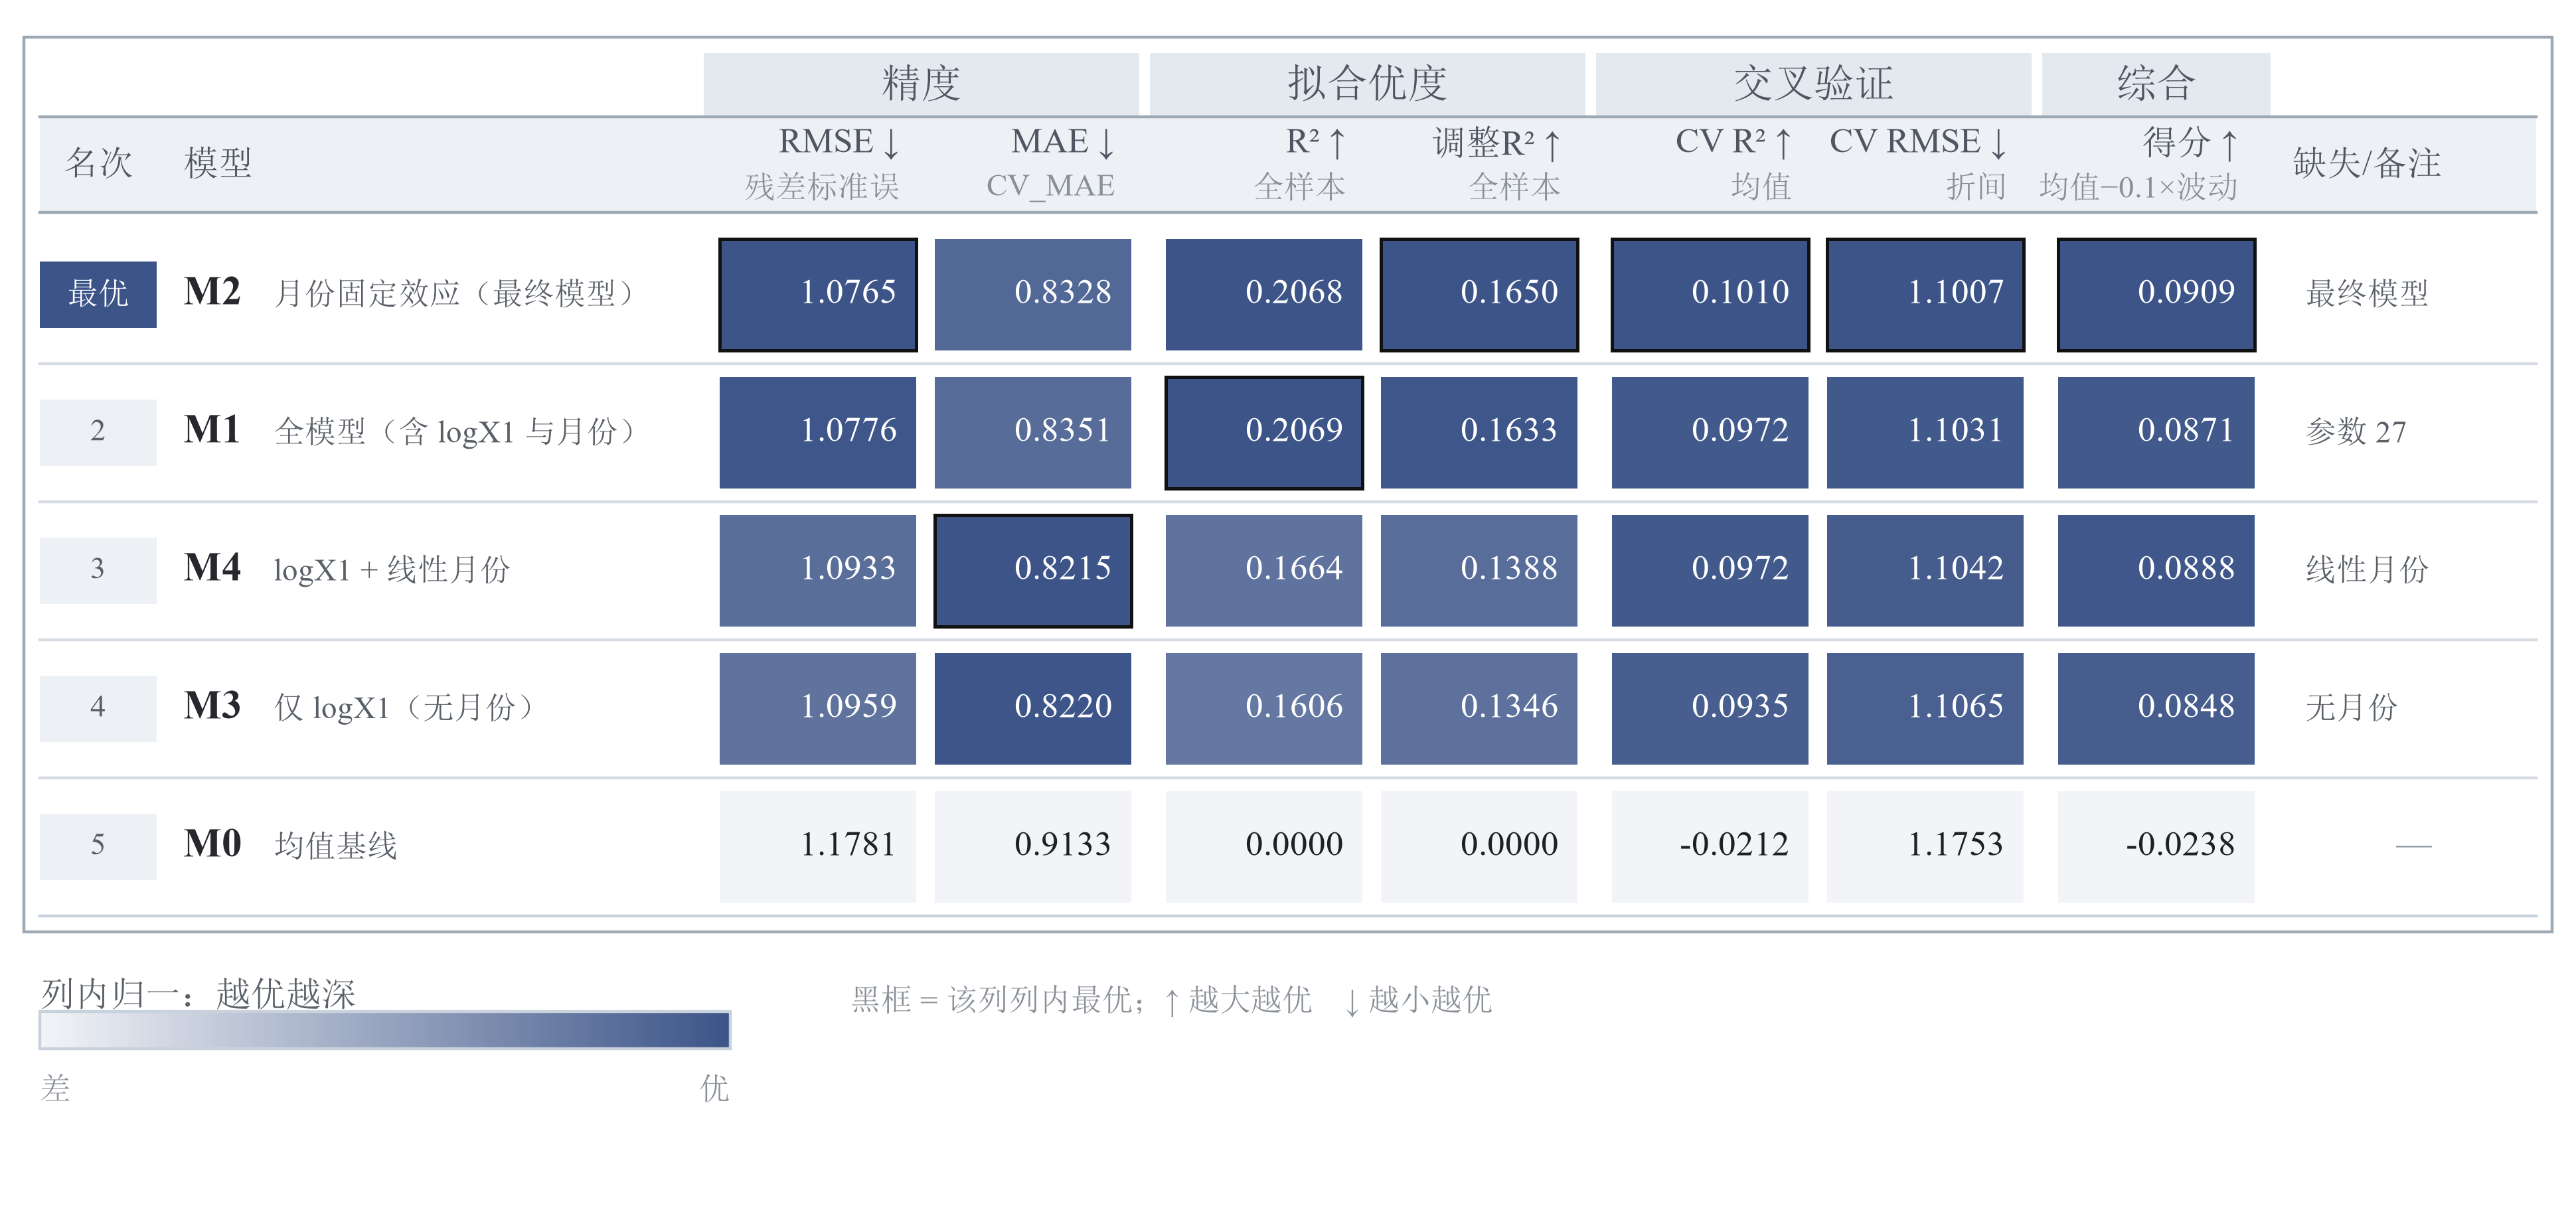
\includegraphics[width=0.74\textwidth]{../求解/问题三/结果/图15_模型绩效评分表.png}
  \caption{五种模型的精度、拟合优度、交叉验证与综合得分}
  \label{fig:q3_score}
\end{figure}

\subsubsection{共线与残差诊断}

表\ref{tab:q3_diag}把共线与残差证据集中列出。M1 的最大 VIF 为 142.99，出现在 10 月；粉丝规模的 VIF 为 124.91；标准化条件数为 48.52，超过 30 的严重阈值。月份哑变量的 VIF 自 3 月起快速上升，到 10 月达到峰值，与粉丝规模的 VIF 互为镜像，说明二者在争抢同一段变异。增量 $F$ 检验显示，在已含月份固定效应的模型中加入粉丝规模，$F$ 值仅 0.0495、$p$ 值 0.824，几乎不增加任何解释力。M2 剔除粉丝规模后，最大 VIF 降至 3.232、条件数降至 6.356，共线问题基本消除；GVIF 方面，粉丝规模的 $\mathrm{GVIF}^{1/2}$ 为 11.176，远超阈值 2.24，其余变量组均低于 1.28。

\begin{longtable}{>{\centering\arraybackslash}p{0.28\textwidth}>{\centering\arraybackslash}p{0.23\textwidth}>{\centering\arraybackslash}p{0.11\textwidth}>{\centering\arraybackslash}p{0.26\textwidth}}
  \caption{共线性与残差诊断}
  \label{tab:q3_diag} \\
  \toprule
  诊断项 & 对象 & 数值 & 判断 \\
  \midrule
  \endfirsthead
  \caption{共线性与残差诊断（续）} \\
  \toprule
  诊断项 & 对象 & 数值 & 判断 \\
  \midrule
  \endhead
  \bottomrule
  \endfoot
  M1 最大 VIF & 全部解释变量 & 142.994 & 超过 10，严重共线 \\
  M1 VIF & $\log X_1$ & 124.905 & 超过 10，严重共线 \\
  M1 条件数 & 标准化设计矩阵 & 48.519 & 超过 30，数值不稳定 \\
  增量 $F$ 统计量 & 在 M2 中加入 $\log X_1$ & 0.0495 & 增量贡献极小 \\
  增量 $F$ 检验 $p$ 值 & 同上 & 0.824 & 不显著，系数不可识别 \\
  $R^2(\log X_1\sim\text{月份})$ & 月间趋势 & 0.9917 & 粉丝规模几乎由月份决定 \\
  月内方差占比 & 组内变异 & 0.0083 & 低于 0.05，月内信息不足 \\
  M2 最大 VIF & 全部解释变量 & 3.232 & 低于 5，可接受 \\
  M2 条件数 & 标准化设计矩阵 & 6.356 & 低于 30，通过 \\
  $\mathrm{GVIF}^{1/2}$ & $\log X_1$ & 11.176 & 超过阈值 2.24 \\
  $\mathrm{GVIF}^{1/2}$ & 其余变量组 & 1.018--1.278 & 均低于 2.24 \\
  Jarque--Bera & M2 残差 & 120.360 & $p<0.001$，残差非正态 \\
  Breusch--Pagan & M2 残差 & 54.737 & $p=0.0005$，存在异方差 \\
  White & M2 残差 & 266.519 & $p=0.030$，存在异方差 \\
  Ramsey RESET & M2 & 2.845 & $p=0.059$，未检出设定误差 \\
  Durbin--Watson & M2 & 2.052 & 接近 2，无强自相关 \\
  Cook 距离最大值 & M2 & 0.0377 & 远小于 1，无强影响点 \\
  高杠杆点个数 & M2 & 10 & 阈值 $2p/n=0.104$ \\
\end{longtable}

图\ref{fig:q3_vif}直观展示共线处理前后的差异。左图中粉丝规模与 6 月至 12 月的月份哑变量全部越过 10 的参考线，最高接近 143；右图中最终模型的全部变量都落在 5 以下，最高的月份变量仅为 3.23。这说明剔除粉丝规模并非损失信息，而是把重复计数的时间维度合并为一个，使剩余系数可以稳定估计。

\begin{figure}[ht]
  \centering
  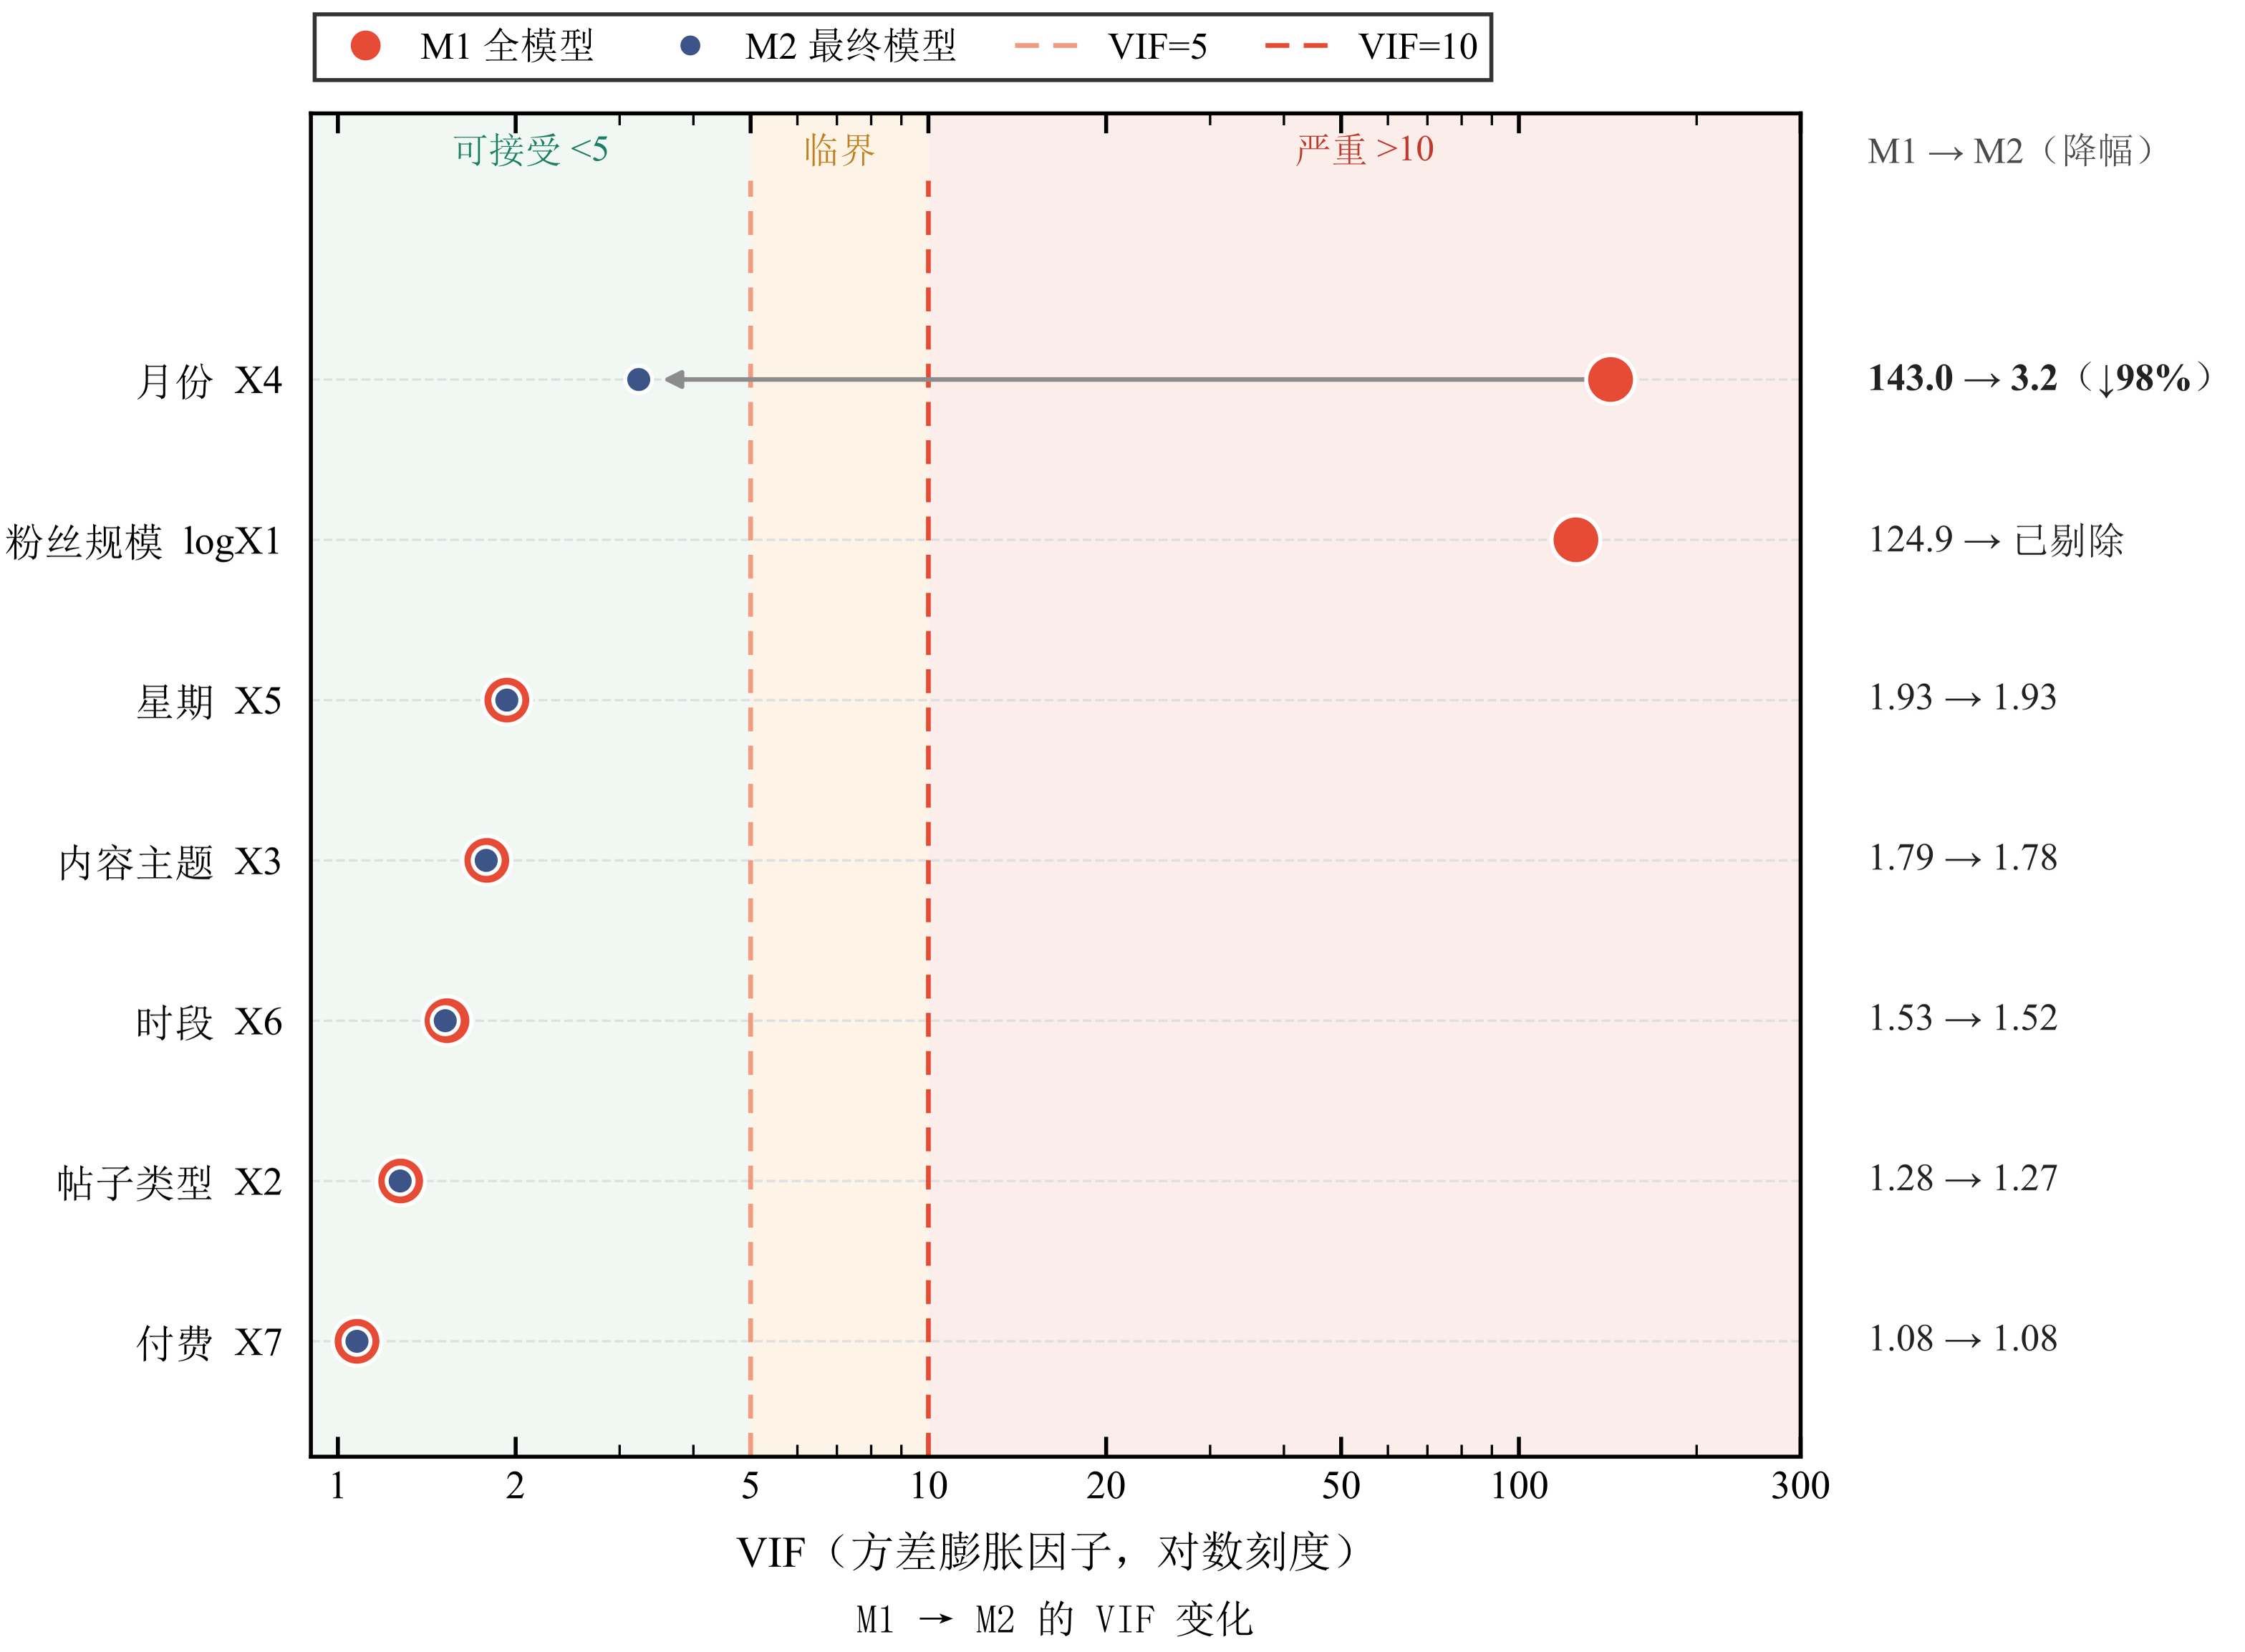
\includegraphics[width=0.68\textwidth]{../求解/问题三/结果/图7_共线性诊断.png}
  \caption{全模型与最终模型的方差膨胀因子}
  \label{fig:q3_vif}
\end{figure}

最终模型 M2 的系数如表\ref{tab:q3_final}所示。常数项 9.2468 对应参照组合（Photo、主题 1、1 月、周一、上午、自然）的基线对数曝光。Status 的系数为 1.1538、$p$ 值小于 0.001，折算为 $e^{1.1538}=3.17$ 倍；Video 为 1.5896、$p$ 值 0.0001，折算为 4.90 倍；Link 为 0.1215、$p$ 值 0.643，折算为 1.13 倍且不显著。主题 2 与主题 3 分别为 $-0.4784$ 与 $-0.3147$，折算为 0.62 倍与 0.73 倍。付费系数为 0.3374、$p$ 值 0.005，折算为 1.40 倍。月份与星期的系数为控制变量，完整估计见表\ref{tab:q3_final}；其中 2 月、4 月为正，10 月为负，其余月份与全部星期、时段系数均不显著。

\begin{longtable}{>{\centering\arraybackslash}p{0.17\textwidth}>{\centering\arraybackslash}p{0.085\textwidth}>{\centering\arraybackslash}p{0.085\textwidth}>{\centering\arraybackslash}p{0.07\textwidth}>{\centering\arraybackslash}p{0.07\textwidth}>{\centering\arraybackslash}p{0.08\textwidth}>{\centering\arraybackslash}p{0.08\textwidth}>{\centering\arraybackslash}p{0.08\textwidth}}
  \caption{最终模型 M2 系数表}
  \label{tab:q3_final} \\
  \toprule
  变量 & 系数 & HC3\newline 标准误 & $t$ 值 & $p$ 值 & CI 下限 & CI 上限 & VIF \\
  \midrule
  \endfirsthead
  \caption{最终模型 M2 系数表（续）} \\
  \toprule
  变量 & 系数 & HC3\newline 标准误 & $t$ 值 & $p$ 值 & CI 下限 & CI 上限 & VIF \\
  \midrule
  \endhead
  \bottomrule
  \endfoot
  常数项 & 9.247 & 0.205 & 45.062 & $<$0.001 & 8.844 & 9.650 & — \\
  类型 Status & 1.154 & 0.124 & 9.339 & $<$0.001 & 0.911 & 1.397 & 1.275 \\
  类型 Link & 0.122 & 0.262 & 0.464 & 0.643 & $-0.393$ & 0.636 & 1.136 \\
  类型 Video & 1.590 & 0.402 & 3.958 & $<$0.001 & 0.800 & 2.379 & 1.063 \\
  主题 2 & $-0.478$ & 0.135 & $-3.540$ & $<$0.001 & $-0.744$ & $-0.213$ & 1.783 \\
  主题 3 & $-0.315$ & 0.134 & $-2.353$ & 0.019 & $-0.578$ & $-0.052$ & 1.527 \\
  月份 2 & 0.877 & 0.304 & 2.886 & 0.004 & 0.280 & 1.473 & 2.039 \\
  月份 3 & $-0.041$ & 0.310 & $-0.134$ & 0.894 & $-0.650$ & 0.567 & 2.543 \\
  月份 4 & 0.381 & 0.177 & 2.154 & 0.032 & 0.033 & 0.728 & 2.835 \\
  月份 5 & 0.191 & 0.171 & 1.116 & 0.265 & $-0.145$ & 0.527 & 2.362 \\
  月份 6 & 0.149 & 0.185 & 0.806 & 0.421 & $-0.214$ & 0.513 & 2.820 \\
  月份 7 & 0.313 & 0.190 & 1.648 & 0.100 & $-0.060$ & 0.687 & 2.971 \\
  月份 8 & 0.112 & 0.248 & 0.451 & 0.652 & $-0.376$ & 0.600 & 2.306 \\
  月份 9 & $-0.126$ & 0.188 & $-0.671$ & 0.503 & $-0.495$ & 0.243 & 2.426 \\
  月份 10 & $-0.471$ & 0.214 & $-2.206$ & 0.028 & $-0.891$ & $-0.051$ & 3.232 \\
  月份 11 & 0.036 & 0.196 & 0.181 & 0.856 & $-0.349$ & 0.420 & 2.808 \\
  月份 12 & $-0.101$ & 0.164 & $-0.616$ & 0.538 & $-0.424$ & 0.222 & 2.851 \\
  星期 2 & 0.094 & 0.198 & 0.475 & 0.635 & $-0.295$ & 0.482 & 1.759 \\
  星期 3 & $-0.019$ & 0.192 & $-0.099$ & 0.921 & $-0.396$ & 0.358 & 1.768 \\
  星期 4 & 0.259 & 0.208 & 1.241 & 0.215 & $-0.151$ & 0.668 & 1.847 \\
  星期 5 & $-0.093$ & 0.177 & $-0.525$ & 0.600 & $-0.441$ & 0.255 & 1.795 \\
  星期 6 & $-0.161$ & 0.185 & $-0.868$ & 0.386 & $-0.525$ & 0.203 & 1.932 \\
  星期 7 & $-0.221$ & 0.175 & $-1.263$ & 0.207 & $-0.566$ & 0.123 & 1.897 \\
  时段 凌晨 & 0.164 & 0.114 & 1.443 & 0.150 & $-0.060$ & 0.388 & 1.318 \\
  时段 下午晚间 & 0.075 & 0.160 & 0.471 & 0.638 & $-0.238$ & 0.389 & 1.520 \\
  付费 & 0.337 & 0.120 & 2.823 & 0.005 & 0.103 & 0.572 & 1.077 \\
\end{longtable}

图\ref{fig:q3_forest}以森林图形式展示主效应。点估计按正负与显著性着色，横轴为 log1p 尺度，右侧标注折算后的倍数与 95\% 置信区间。Status 与 Video 的区间完全位于 0 的右侧，主题 2 与主题 3 的区间完全位于 0 的左侧，付费的区间也整体为正；Link 的区间跨越 0，对应 $p$ 值 0.643。Video 的区间最宽，上界接近 2.38，这是仅 7 条视频帖带来的必然结果，解读时应强调方向而非精确倍数。

\begin{figure}[ht]
  \centering
  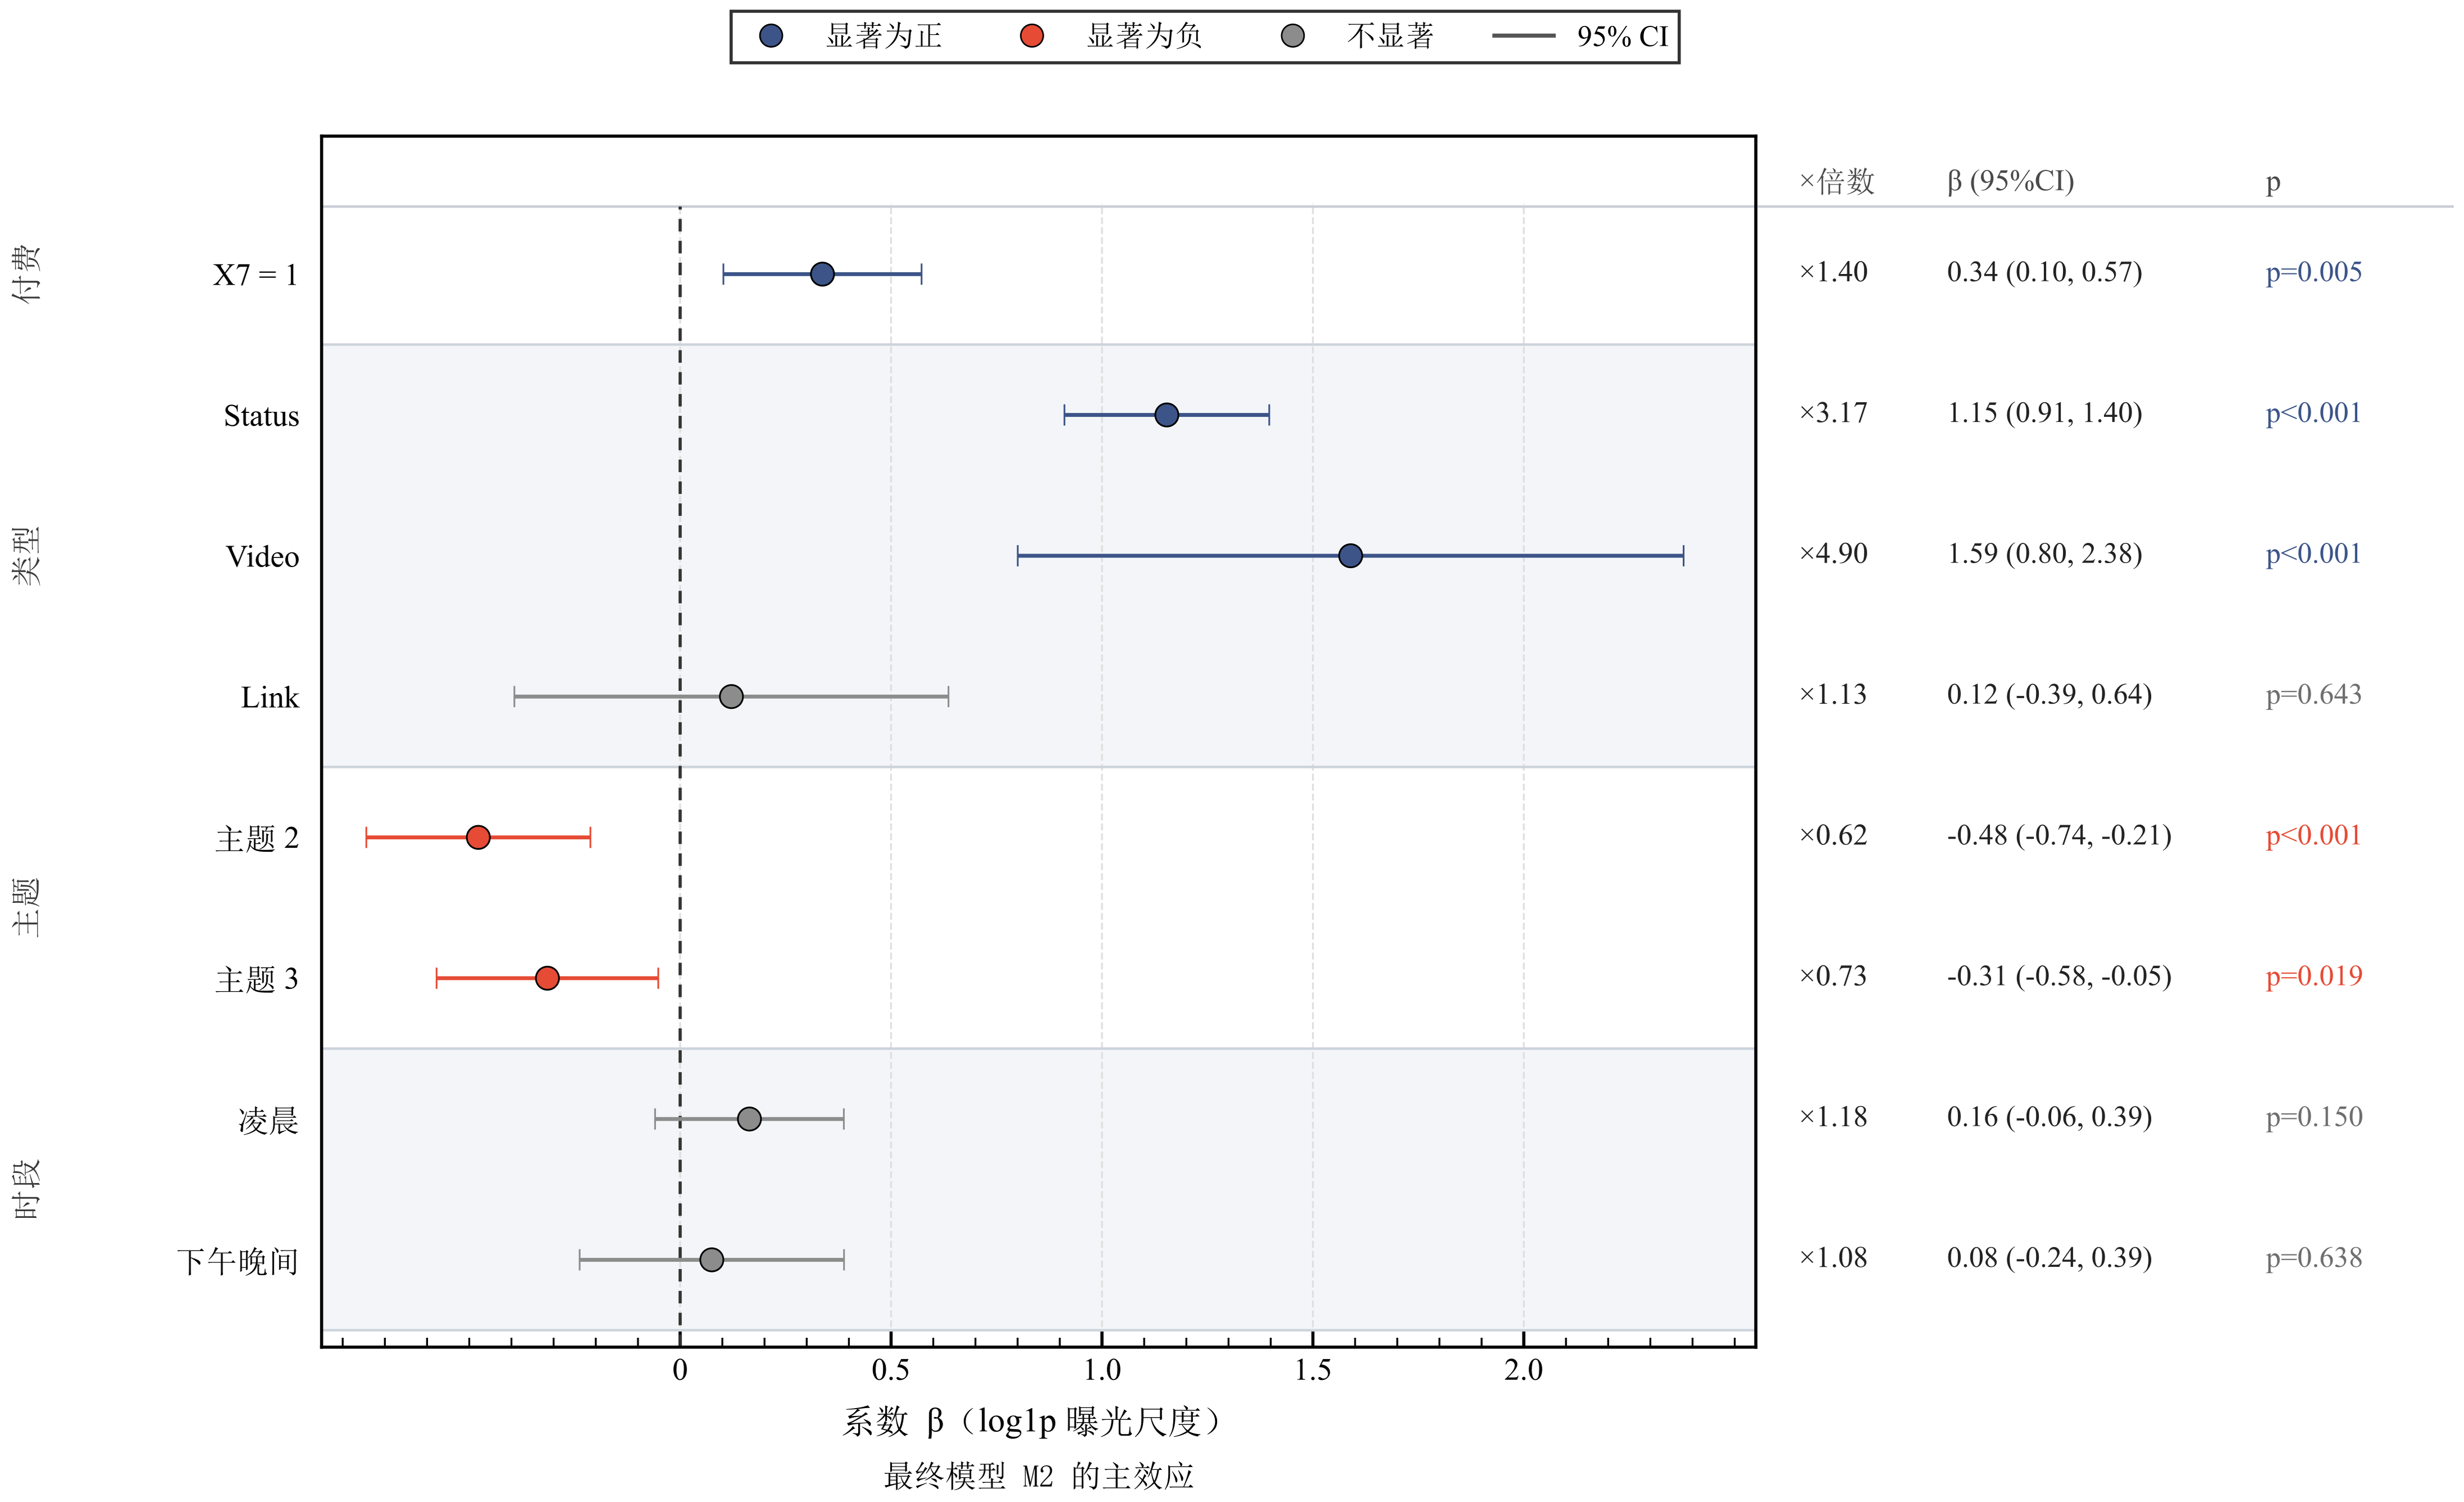
\includegraphics[width=0.70\textwidth]{../求解/问题三/结果/图6_最终模型系数森林图.png}
  \caption{最终模型主效应系数与 95\% 置信区间}
  \label{fig:q3_forest}
\end{figure}

表\ref{tab:q3_diag}的下半部分报告残差诊断。Jarque--Bera 统计量为 120.36、$p$ 值小于 0.001，残差仍偏离正态；Breusch--Pagan 统计量为 54.74、$p$ 值 0.0005，White 统计量 266.52、$p$ 值 0.030，两项都拒绝同方差。这正是采用 HC3 标准误的理由。Ramsey RESET 的 $F$ 值为 2.845、$p$ 值 0.059，在 5\% 水平未检出函数形式误设；Durbin--Watson 为 2.052，接近 2；Cook 距离最大值为 0.0377，远小于 1，说明没有单条帖子主导估计。按 $4/n=0.0080$ 的常用参考线，有 30 个观测超过该线，但最大 Cook 距离仍不足 0.04，属于局部影响而非全局主导；杠杆值超过 $2p/n=0.104$ 的观测有 10 个。

\begin{figure}[ht]
  \centering
  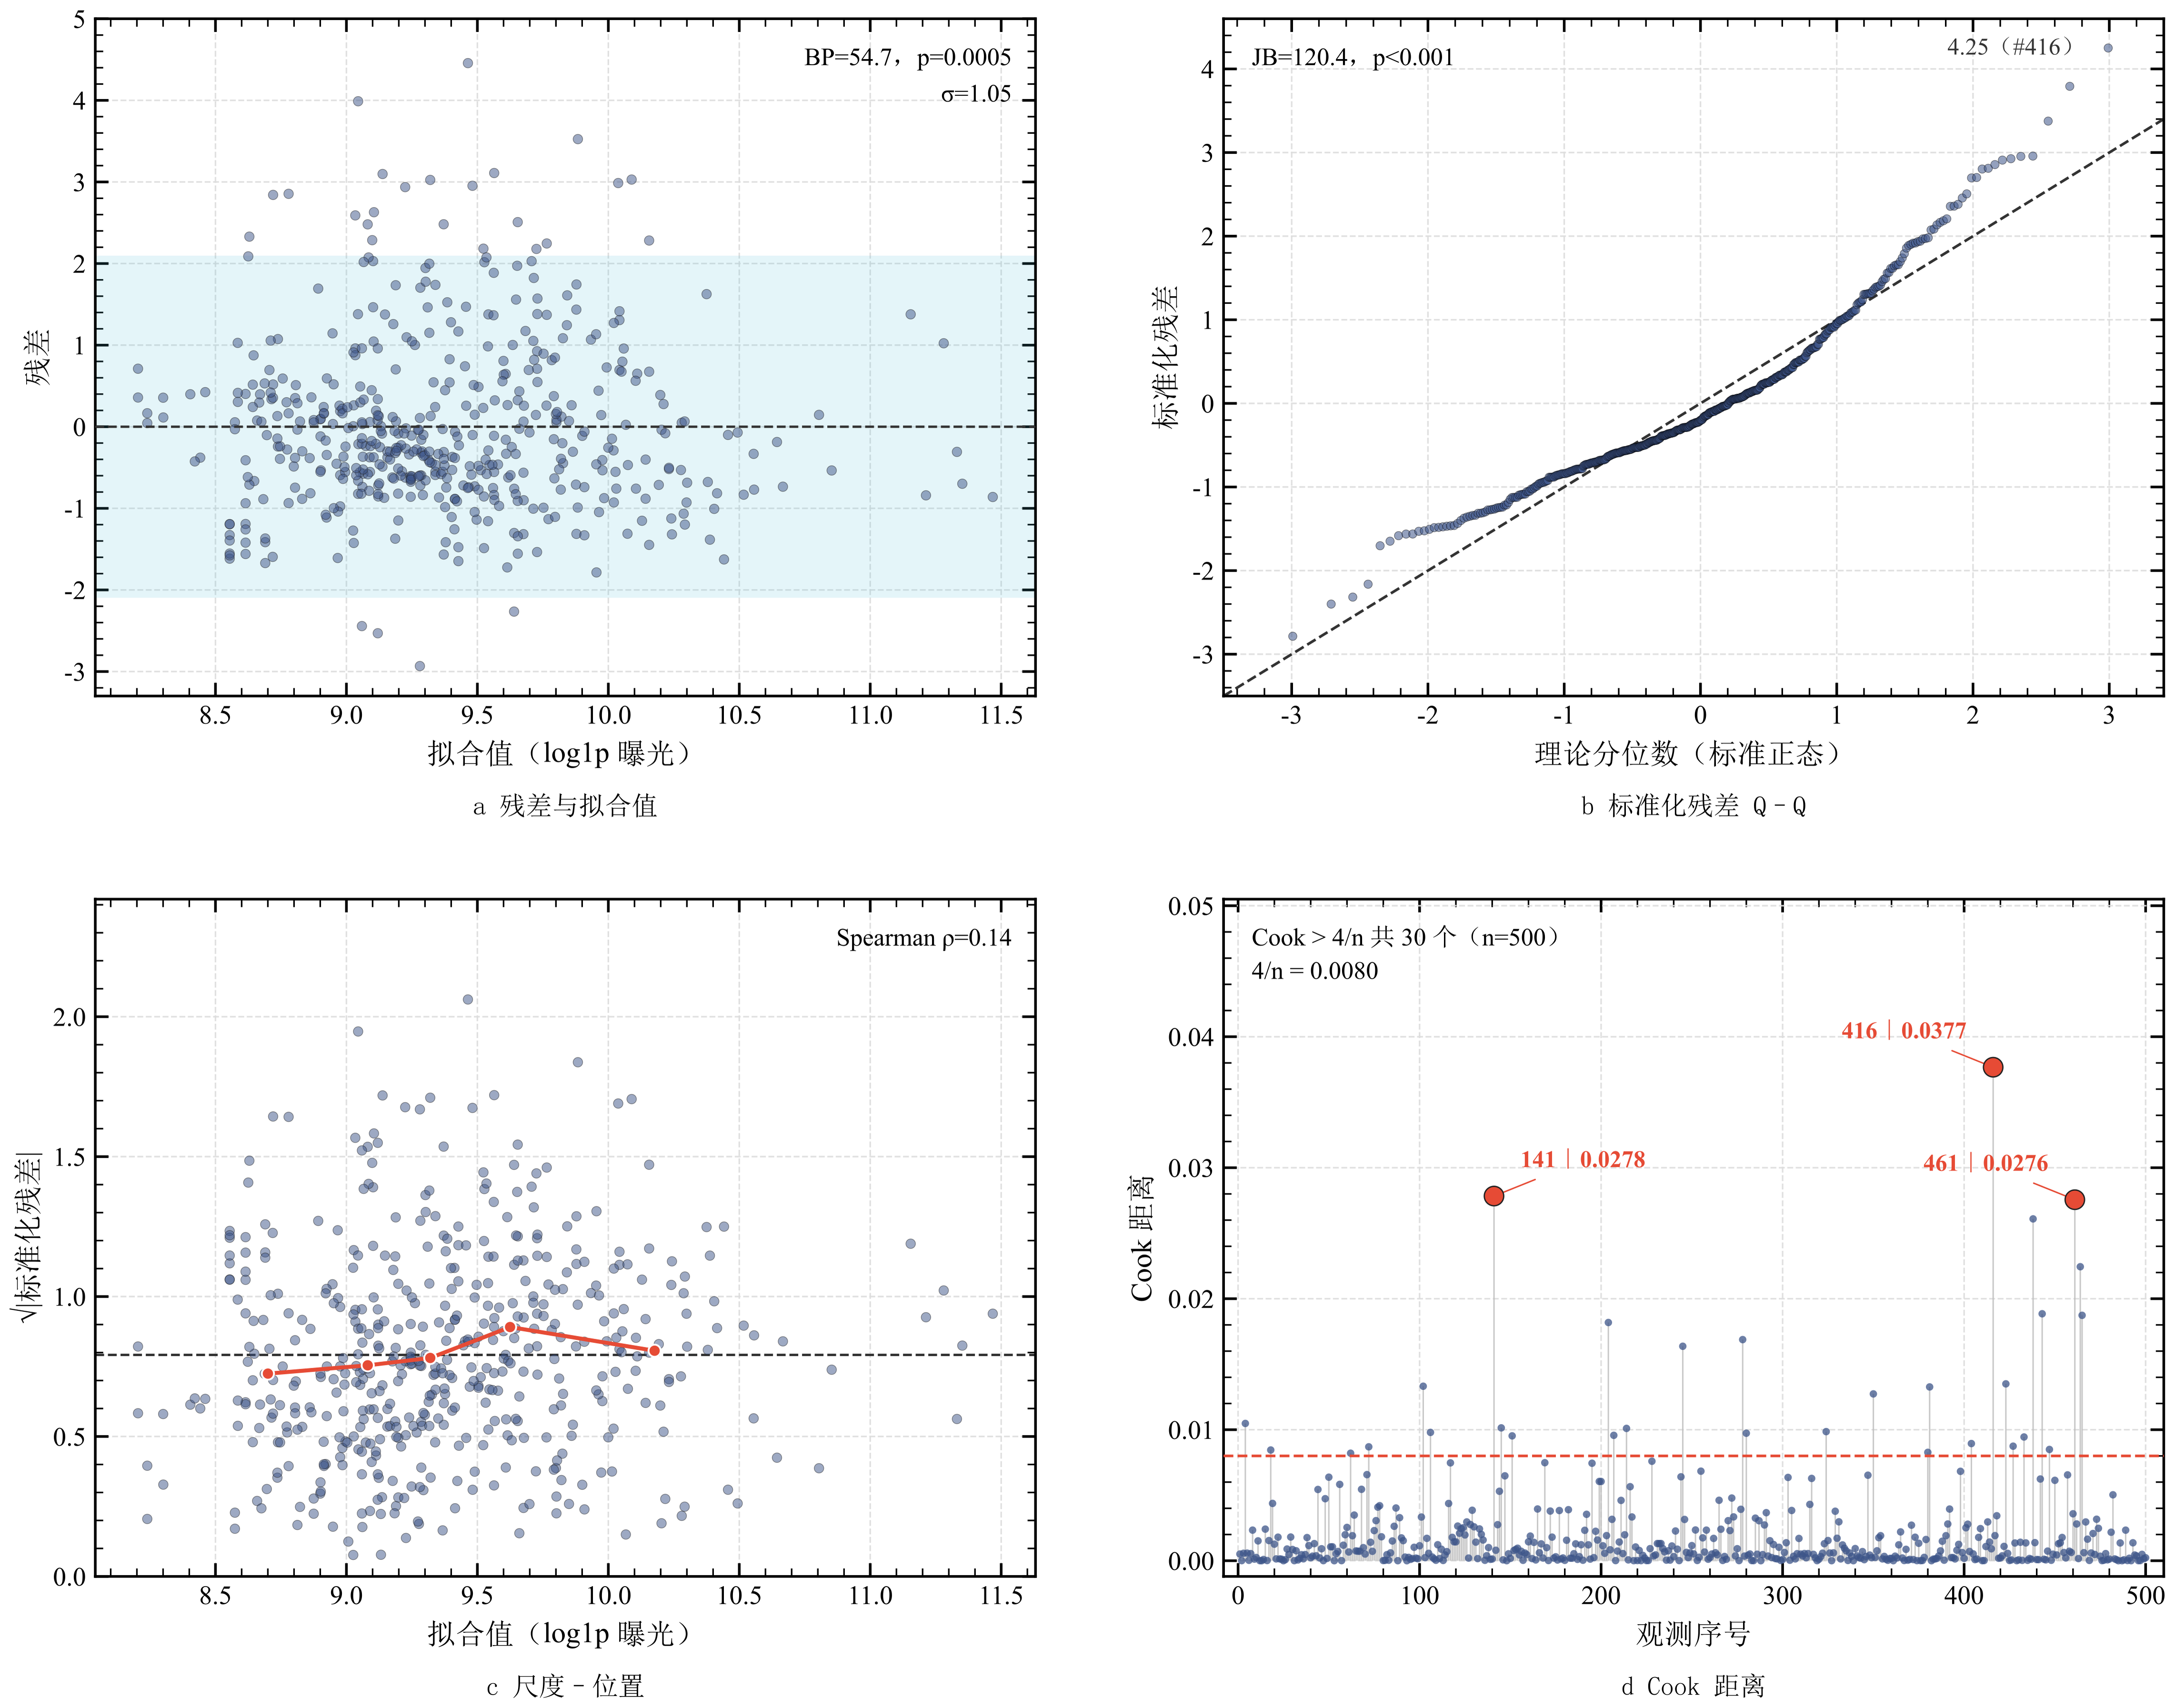
\includegraphics[width=0.68\textwidth]{../求解/问题三/结果/图8_残差诊断.png}
  \caption{最终模型残差诊断}
  \label{fig:q3_resid}
\end{figure}

图\ref{fig:q3_resid}把残差结构可视化。残差对拟合值呈水平带状分布，均值接近 0，但在低拟合值区略厚；Q--Q 图两端偏离参考线，对应少数极端曝光帖；尺度—位置图的平滑线基本水平，Spearman 相关仅 0.14，说明异方差主要来自尾部而非系统性趋势；Cook 距离图显示 30 个观测超过 $4/n$ 参考线，最高为编号 416 的 0.0377，其余依次为 141 的 0.0278 与 461 的 0.0276。整体看，残差没有呈现明显的非线性或漏斗形，HC3 标准误足以应对剩余的异方差。

\subsubsection{拟合优度与方差分解}

图\ref{fig:q3_cv}对比样本内与交叉验证表现。左图中各模型的 CV $R^2$ 都低于样本内 $R^2$，M2 由 0.2068 降至 0.1010，降幅约一半，说明模型存在一定过拟合，但方向仍为正；M1 的降幅更大，M0 的 CV $R^2$ 为 $-0.0212$。右图为 M2 的交叉验证预测与观测对照，点云沿 45 度线分布，但离散程度较大，CV $R^2$ 仅 0.101、RMSE 1.101、MAE 0.833，说明单条帖子的曝光量很难被完全预测，模型的价值在于识别平均效应而非精确点预测。

\begin{figure}[ht]
  \centering
  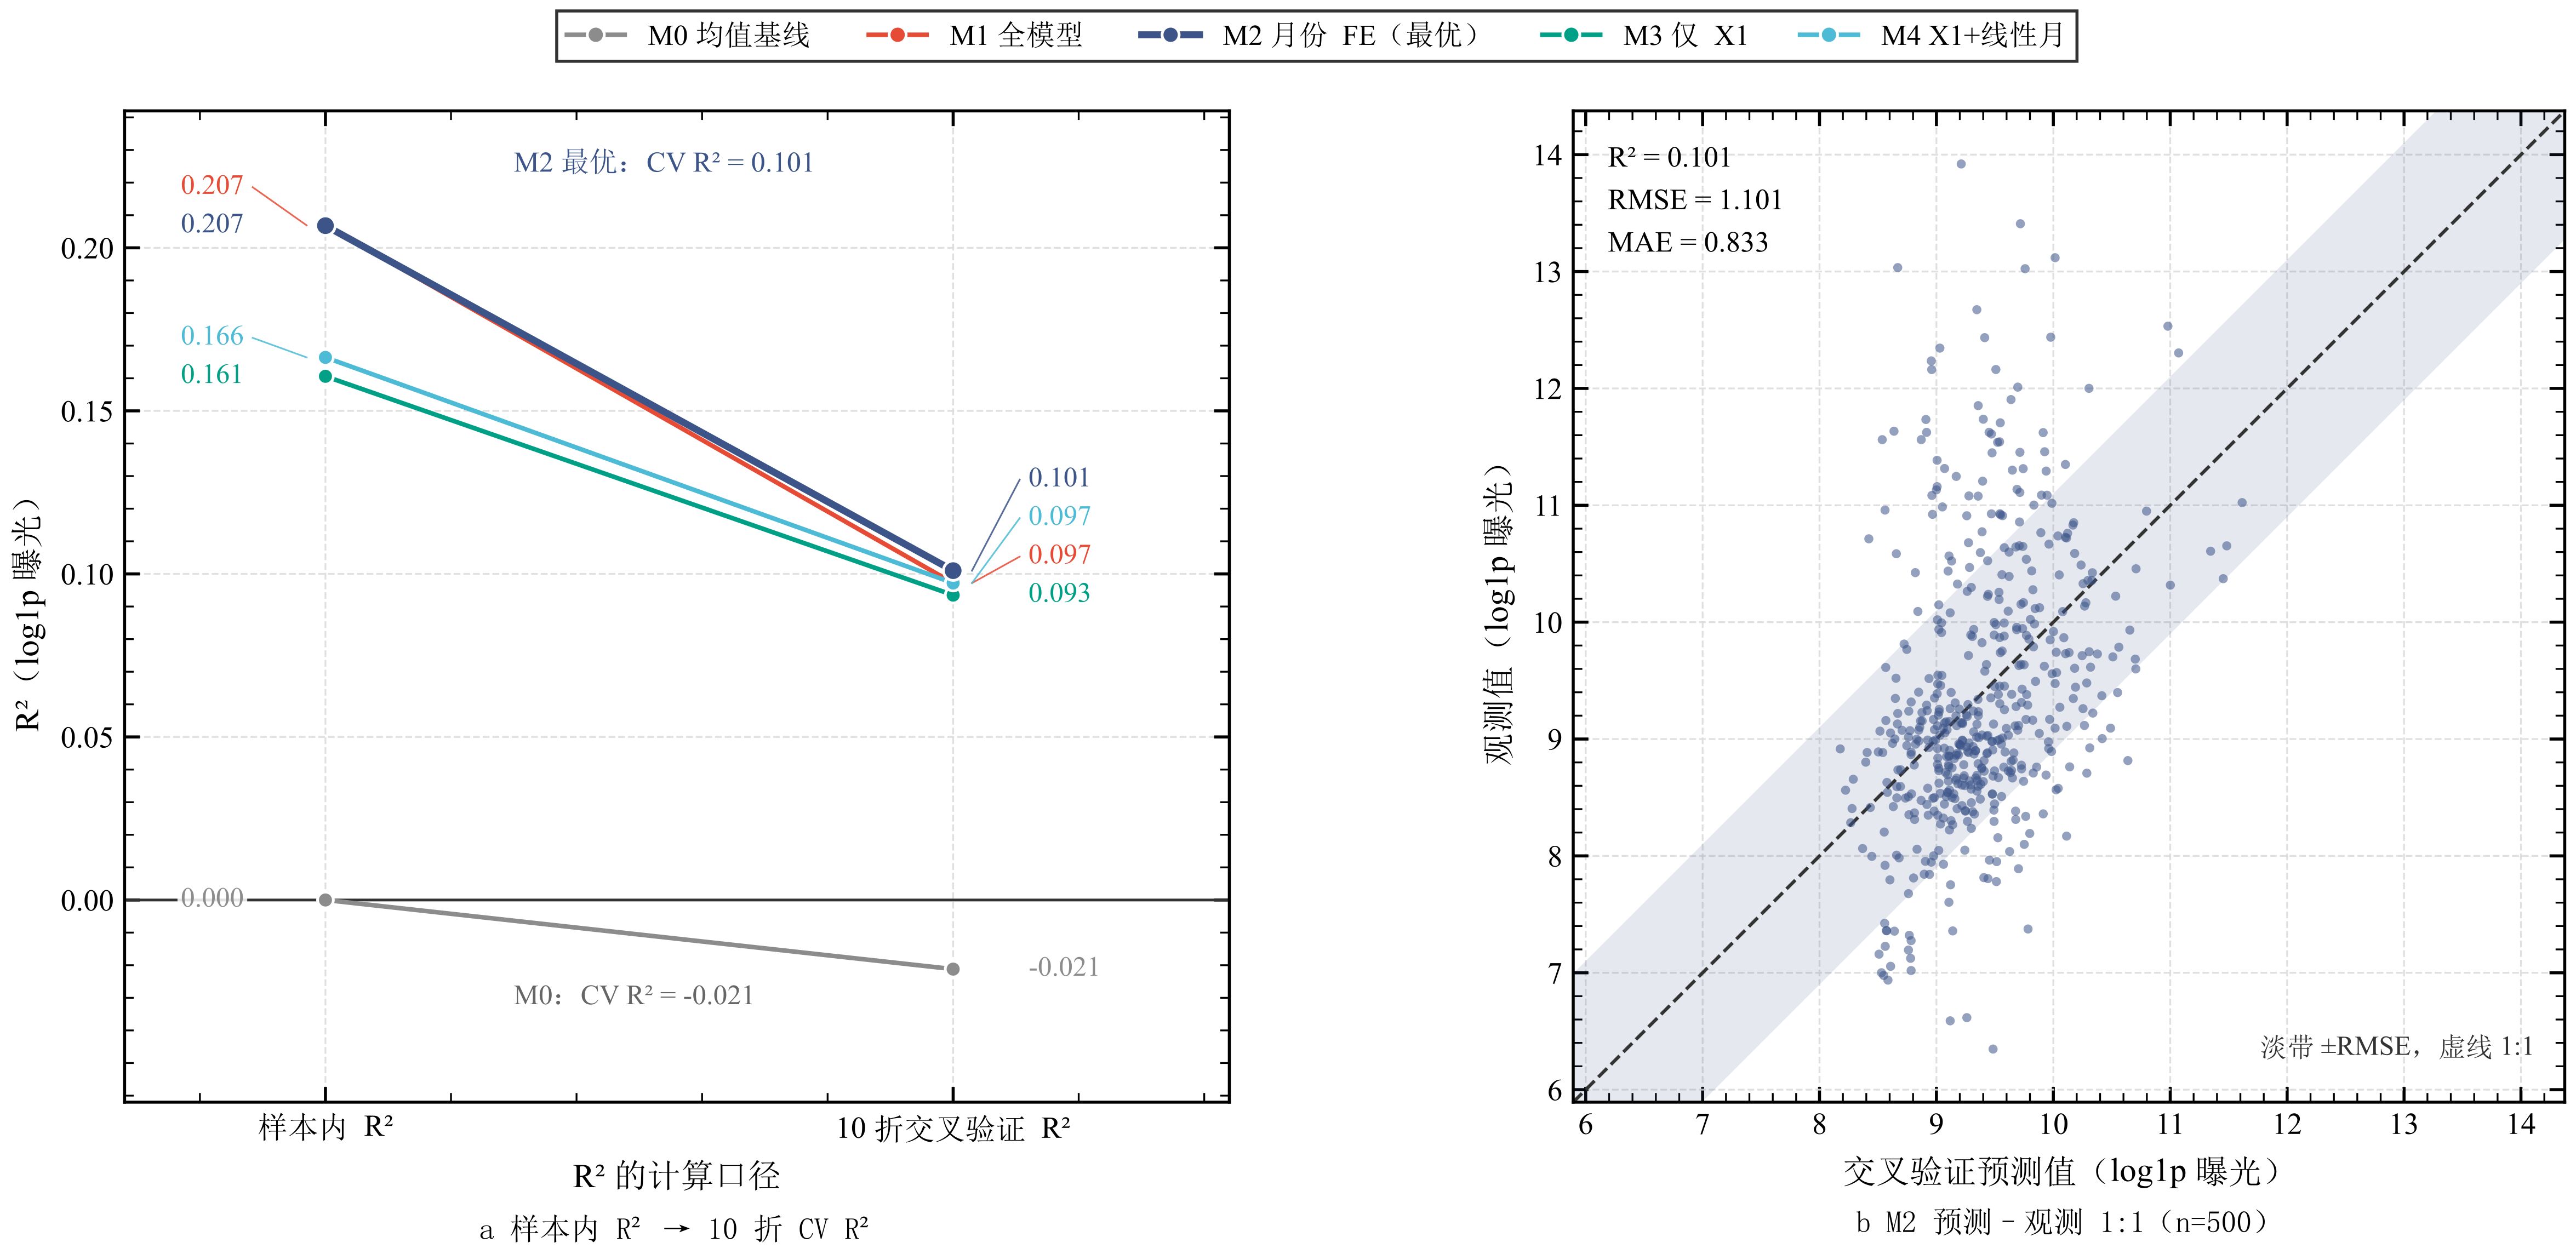
\includegraphics[width=0.74\textwidth]{../求解/问题三/结果/图9_预测能力验证.png}
  \caption{样本内与交叉验证预测能力}
  \label{fig:q3_cv}
\end{figure}

最后给出方差分解。图\ref{fig:q3_shapley}显示，帖子类型 X2 的 Shapley 贡献为 0.0767，占已解释方差的 37.1\%，是单一变量组中最大的；月份 X4 为 0.0579、占 28.0\%；付费 X7 为 0.0244、占 11.8\%；星期 X5 为 0.0236、占 11.4\%；内容主题 X3 为 0.0142、占 6.9\%；时段 X6 为 0.0055、占 2.6\%；粉丝规模 $\log X_1$ 仅为 0.0046、占 2.2\%。按类别合并，发帖决策合计解释 0.1445，占总方差的 14.45\%；账号规模与时间合计解释 0.0624，占 6.24\%；未解释部分为 0.7931，占 79.31\%。发帖决策的贡献是规模与时间的两倍以上，说明可操控的内容与投放选择比账号自然增长更能解释帖子间的曝光差异；但两者合计仍不足总方差的三分之一，绝大多数变异来自未被观测到的推荐算法、受众匹配与传播随机性。

\begin{figure}[ht]
  \centering
  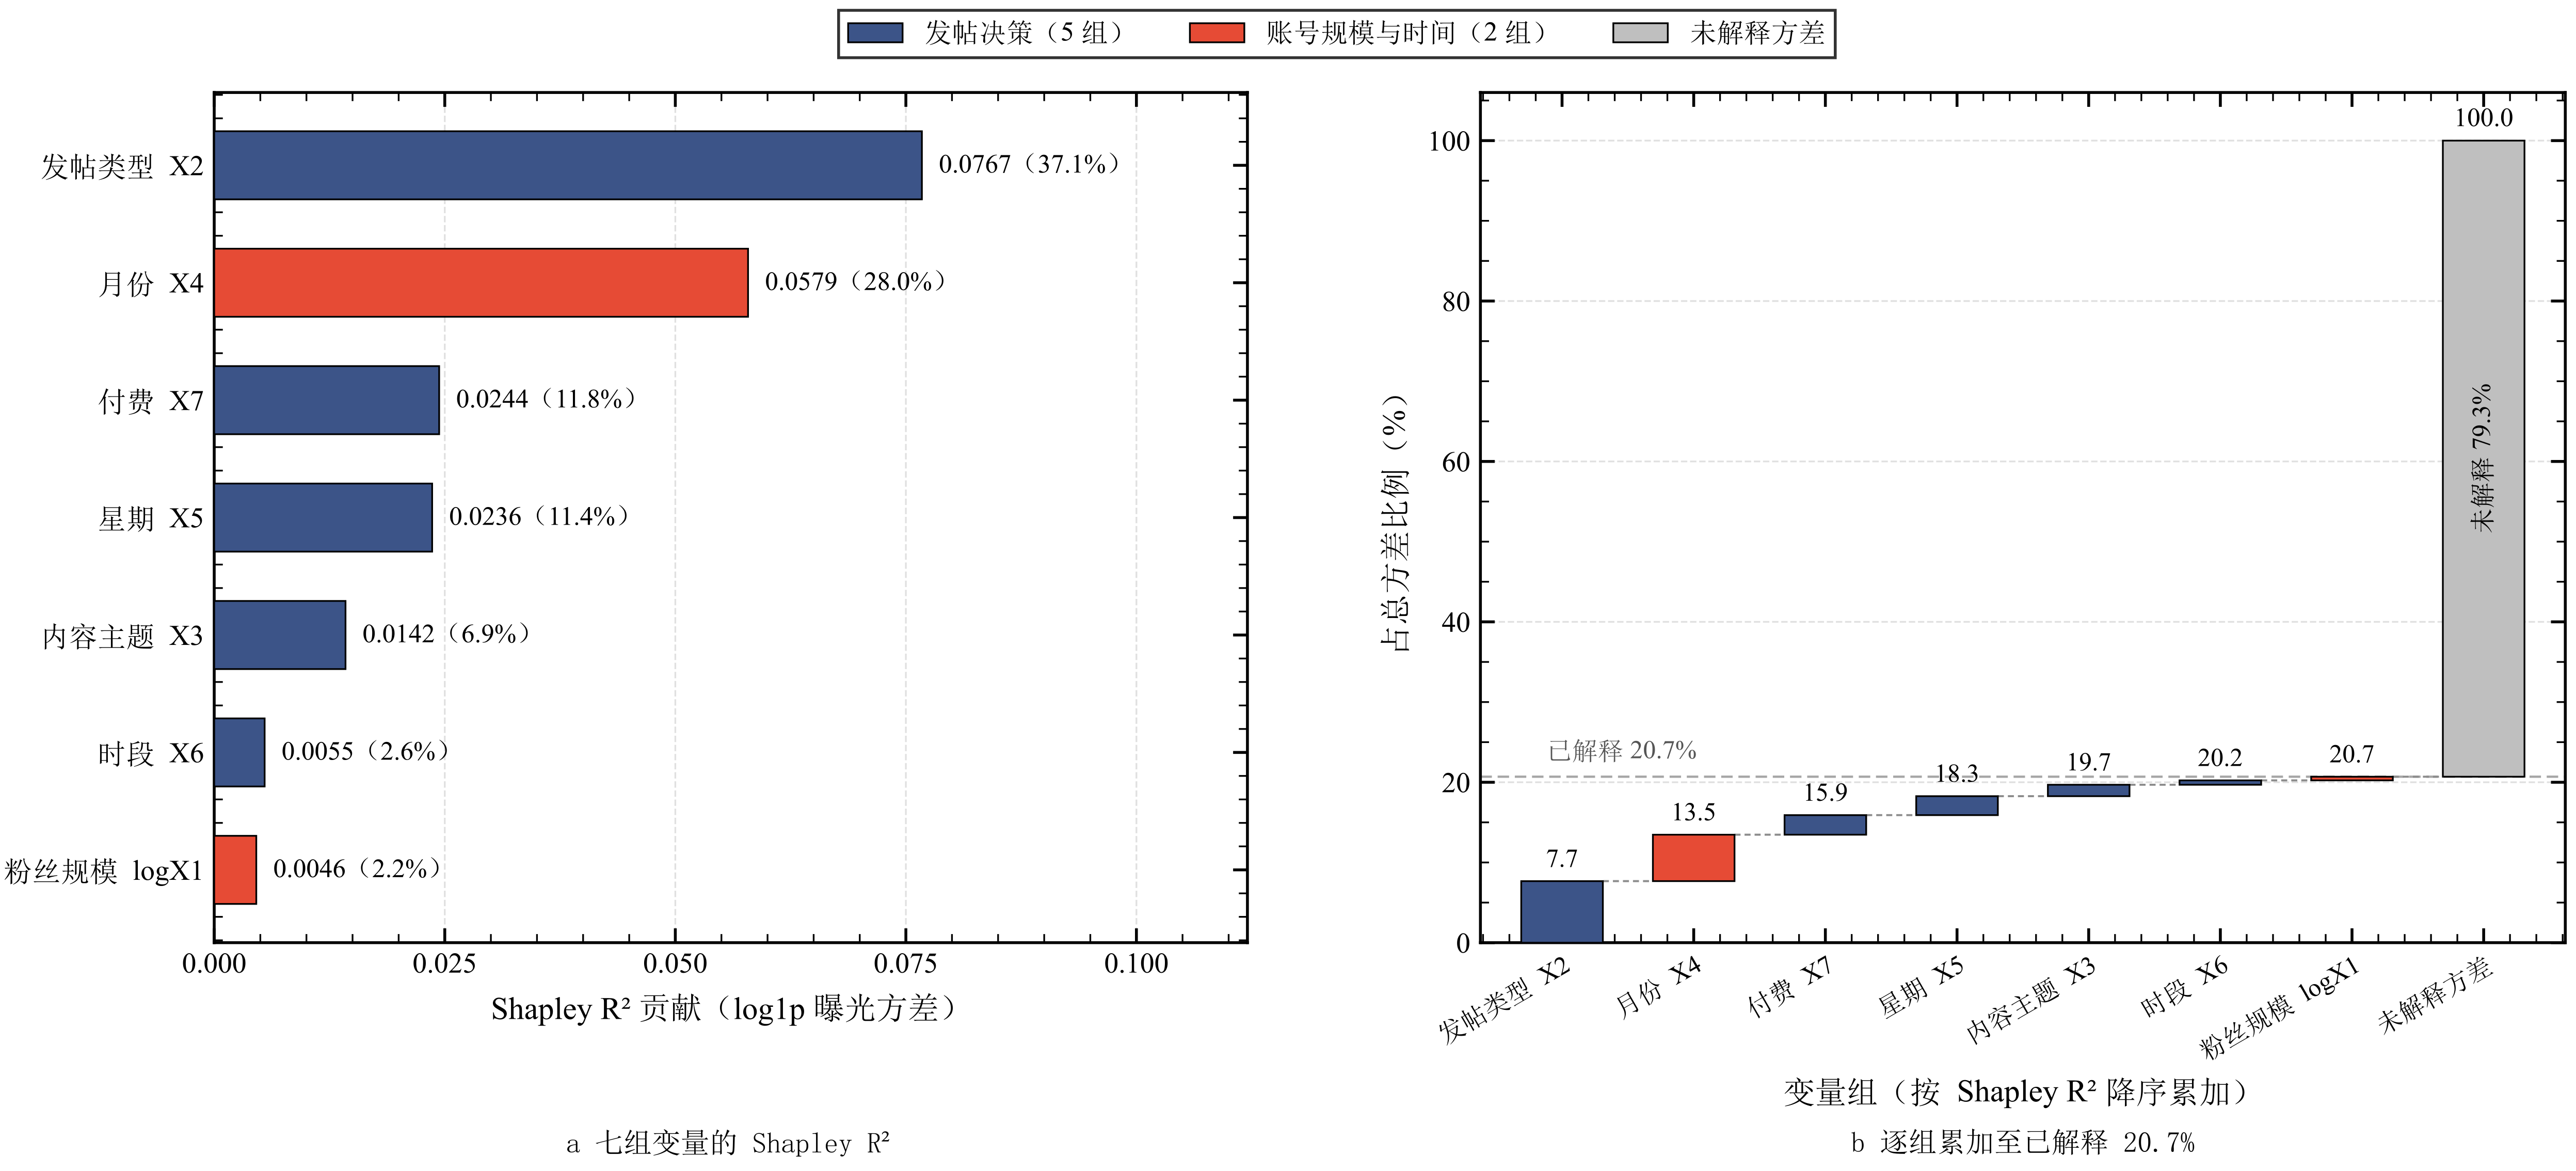
\includegraphics[width=0.74\textwidth]{../求解/问题三/结果/图10_方差贡献Shapley.png}
  \caption{变量组的 Shapley 方差贡献与总方差构成}
  \label{fig:q3_shapley}
\end{figure}

综合以上结果，M1 的粉丝规模系数在共线下不可识别，M2 以月份固定效应替代后共线消除、拟合几乎不变、交叉验证略优。最终模型在整体显著性与残差诊断上基本合格，样本外 $R^2$ 为 0.101，能够支撑平均效应测算，但不适合对单条帖子做精确点预测。发帖决策解释 14.45\% 的曝光方差，是后续效应测算的重点对象。
